\documentclass[a4paper]{article}

% bloc : évite un changement de page
% completemulti : ajoute une case : aucune bonne réponse
%\newcommand{\repRel}{../..}
%\input{\repRel/Style/packages_v2}
%%\input{\repRel/Style/new_style}
%\input{\repRel/Style/macros_SII}
%\input{\repRel/Style/environment_v2}

\usepackage[francais,bloc,completemulti,ensemble]{automultiplechoice}
%\usepackage[francais,bloc,completemulti]{automultiplechoice} 
\usepackage{amsmath}
% ensemble : feuille de questions et feuille de réponse séparées

\usepackage{multicol}

%% Pour le python %%
\usepackage{listingsutf8}

\lstset{language=Python,
  inputencoding=utf8/latin1,
  breaklines=true,
  basicstyle=\ttfamily\small,
  keywordstyle=\bfseries\color{green!40!black},
  commentstyle=\itshape\color{purple!40!black},
  identifierstyle=\color{blue},
  stringstyle=\color{orange},
  upquote = true,
  columns=fullflexible,
  backgroundcolor=\color{gray!10},frame=leftline,rulecolor=\color{gray}}  
  
\definecolor{mygreen}{rgb}{0,0.6,0}

\lstset{
     literate=%
         {é}{{\'e}}1    
         {è}{{\`e}}1    
         {ê}{{\^e}}1    
         {à}{{\`a}}1
         {â}{{\^a}}1		 
         {ô}{{\^o}}1    
         {ù}{{\`u}}1    
         {î}{{\^i}}1    
}
\lstset{inputpath=code}

\usepackage{siunitx}
%\usepackage[utf8x]{inputenc}
%\usepackage[T1]{fontenc}

\begin{document}
\AMCrandomseed{233893}
\setdefaultgroupmode{withoutreplacement} % Mélange des questions groupées

\graphicspath{{../../Banque_SI/04_transmetteurs/images/}}
\element{transmetteurs}{
\begin{question}{tr 01}
Soit le schéma suivant. Déterminer $\dfrac{\omega_{20}}{\omega_{10}}$.
\begin{center}
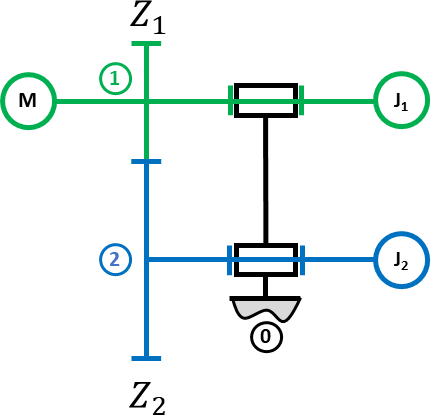
\includegraphics[width=5cm]{fig_01}
\end{center}
\begin{multicols}{4}
	\begin{reponses}	
	\mauvaise{$-\dfrac{Z_2}{Z_1}$}
	\mauvaise{$\dfrac{Z_2}{Z_1}$}
	\bonne{$-\dfrac{Z_1}{Z_2}$}
	\mauvaise{$\dfrac{Z_1}{Z_2}$}
	\end{reponses}
\end{multicols}
\end{question}\\}

\element{transmetteurs}{
\begin{question}{tr 02}
Soit le schéma suivant. Déterminer $\dfrac{\omega_{10}}{\omega_{20}}$.
\begin{center}
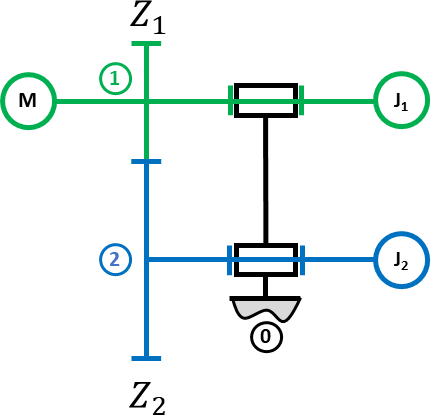
\includegraphics[width=5cm]{fig_01}
\end{center}
\begin{multicols}{4}
	\begin{reponses}	
	\bonne{$-\dfrac{Z_2}{Z_1}$}
	\mauvaise{$\dfrac{Z_2}{Z_1}$}
	\mauvaise{$-\dfrac{Z_1}{Z_2}$}
	\mauvaise{$\dfrac{Z_1}{Z_2}$}
	\end{reponses}
\end{multicols}
\end{question}\\}

\element{transmetteurs}{
\begin{question}{tr 03}
Soit le schéma suivant. Déterminer $\dfrac{\omega_{20}}{\omega_{10}}$.
\begin{center}
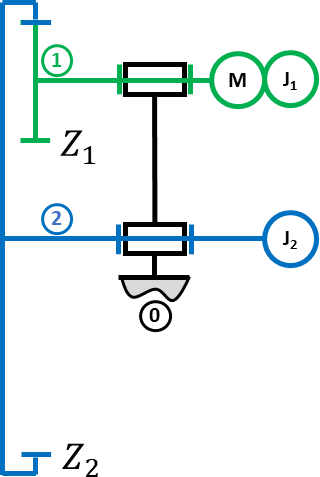
\includegraphics[width=5cm]{fig_02}
\end{center}
\begin{multicols}{4}
	\begin{reponses}	
	\mauvaise{$\dfrac{Z_2}{Z_1}$}
	\mauvaise{$-\dfrac{Z_2}{Z_1}$}
	\mauvaise{$-\dfrac{Z_1}{Z_2}$}
	\bonne{$\dfrac{Z_1}{Z_2}$}
	\end{reponses}
\end{multicols}
\end{question}\\}

\element{transmetteurs}{
\begin{question}{tr 04}
Soit le schéma suivant. Déterminer $\dfrac{\omega_{10}}{\omega_{20}}$.
\begin{center}
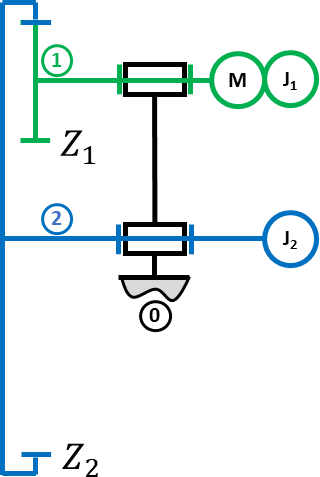
\includegraphics[width=5cm]{fig_02}
\end{center}
\begin{multicols}{4}
	\begin{reponses}	
	\bonne{$-\dfrac{Z_2}{Z_1}$}
	\mauvaise{$\dfrac{Z_2}{Z_1}$}
	\mauvaise{$\dfrac{Z_1}{Z_2}$}
	\mauvaise{$-\dfrac{Z_1}{Z_2}$}
	\end{reponses}
\end{multicols}
\end{question}\\}


\element{transmetteurs}{
\begin{question}{tr 05}
Soit le schéma suivant. Déterminer $\dfrac{\omega_{20}}{\omega_{10}}$.
\begin{center}
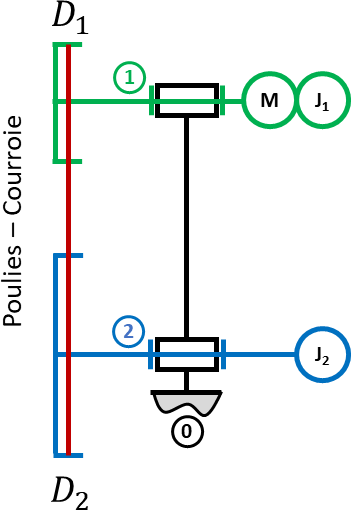
\includegraphics[width=5cm]{fig_03}
\end{center}
\begin{multicols}{4}
	\begin{reponses}	
	\mauvaise{$\dfrac{D_2}{D_1}$}
	\mauvaise{$-\dfrac{D_2}{D_1}$}
	\mauvaise{$-\dfrac{D_1}{D_2}$}
	\bonne{$\dfrac{D_1}{D_2}$}
	\end{reponses}
\end{multicols}
\end{question}\\}

\element{transmetteurs}{
\begin{question}{tr 06}
Soit le schéma suivant. Déterminer $\dfrac{\omega_{10}}{\omega_{20}}$.
\begin{center}
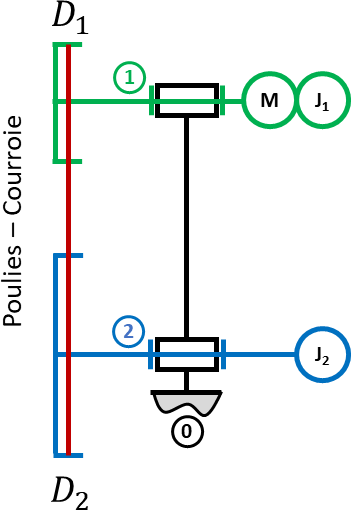
\includegraphics[width=5cm]{fig_03}
\end{center}
\begin{multicols}{4}
	\begin{reponses}	
	\mauvaise{$-\dfrac{D_2}{D_1}$}
	\bonne{$\dfrac{D_2}{D_1}$}
	\mauvaise{$\dfrac{D_1}{D_2}$}
	\mauvaise{$-\dfrac{D_1}{D_2}$}
	\end{reponses}
\end{multicols}
\end{question}\\}



\element{transmetteurs}{
\begin{question}{tr 07}
On note $v$ la vitesse de la charge $M$ selon la direction verticale. Exprimer $v$ en fonction de 
$\omega_{10}$ (en valeur absolue).
\begin{center}
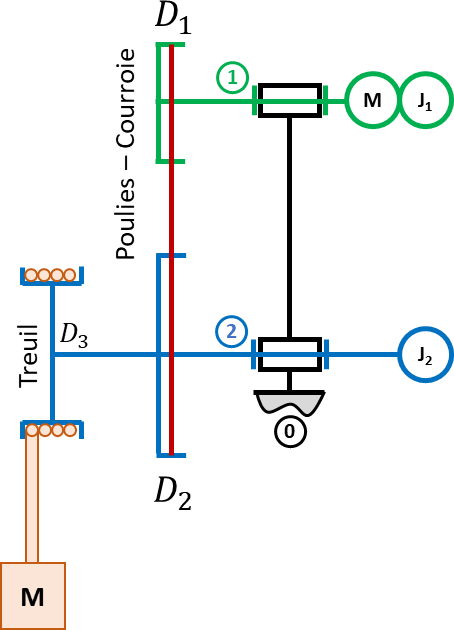
\includegraphics[width=5cm]{fig_04}
\end{center}
\begin{multicols}{4}
	\begin{reponses}	
	\mauvaise{$v = \dfrac{D_2 }{D_1 D_3} \omega_{10}$}
	\mauvaise{$v = \dfrac{D_2 D_3 }{D_1}\omega_{10}$}
	\mauvaise{$v = \dfrac{D_1 D_3 }{D_2} \omega_{10}$}
	\bonne{$v = \dfrac{D_1 D_3}{2 D_2 } \omega_{10}$}
	\end{reponses}
\end{multicols}
\end{question}\\}


\element{transmetteurs}{
\begin{question}{tr 08}
On note $v$ la vitesse de la charge $M$ selon la direction horizontale. Exprimer $v$ en fonction de
$\omega_{10}$ (en valeur absolue). On note $m$ le module des roues dentées.
\begin{center}
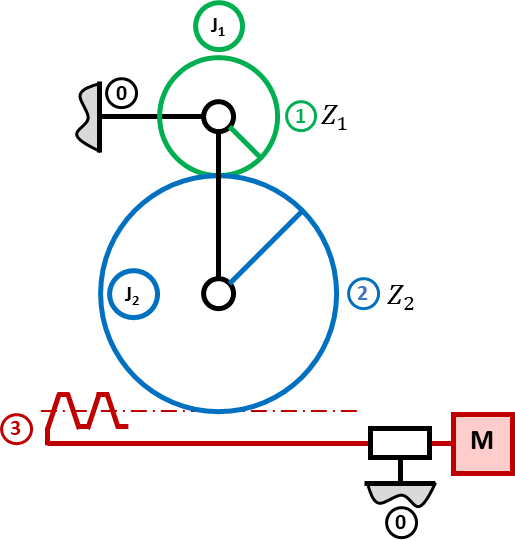
\includegraphics[width=5cm]{fig_05}
\end{center}
\begin{multicols}{4}
	\begin{reponses}	
	\mauvaise{$v = \dfrac{Z_2}{Z_1 } \omega_{10}$}
	\mauvaise{$v = \dfrac{m Z_2}{Z_1 } \omega_{10}$}
	\mauvaise{$v = \dfrac{Z_2^2}{2 Z_1 } \omega_{10}$}
	\bonne{$v = \dfrac{m Z_2^2}{2 Z_1 } \omega_{10}$}
	\end{reponses}
\end{multicols}
\end{question}\\}

\element{transmetteurs}{
\begin{question}{tr 09}
Exprimer $\omega_{10}$ en fonction de $\omega_{30}$ (en valeur absolue). 
\begin{center}
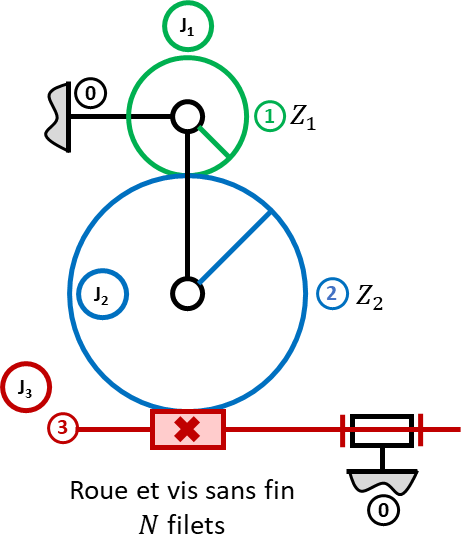
\includegraphics[width=5cm]{fig_06}
\end{center}
\begin{multicols}{4}
	\begin{reponses}	
	\mauvaise{$\omega_{10} = \dfrac{Z_2^2}{NZ_1}  \omega_{30}$}
	\mauvaise{$\omega_{10} = \dfrac{N}{Z_2} \dfrac{Z_1}{Z_2} \omega_{30}$}
	\mauvaise{$\omega_{10} =  NZ_1 \omega_{30}$}
	\bonne{$\omega_{10} = \dfrac{N}{Z_1} \omega_{30}$}
	\end{reponses}
\end{multicols}
\end{question}\\}

\element{transmetteurs}{
\begin{question}{tr 10}
On note $v$ la vitesse de la charge $M$ selon la direction horizontale. Exprimer $v$ en fonction de 
$\omega_{10}$ (en valeur absolue). On note $p$ le pas de la vis.
\begin{center}
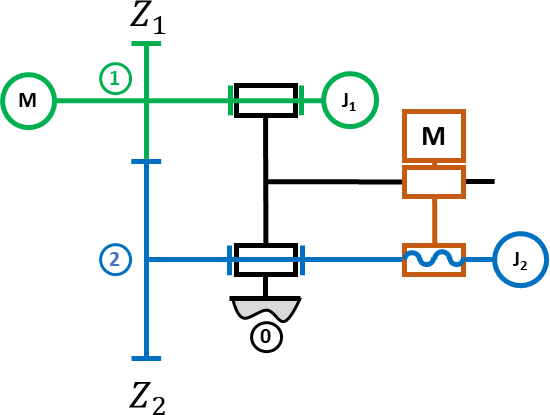
\includegraphics[width=5cm]{fig_07}
\end{center}
\begin{multicols}{4}
	\begin{reponses}	
	\mauvaise{$v = \dfrac{ Z_2  }{ Z_1  p } \omega_{10}$}
	\mauvaise{$v = \dfrac{Z_2 p}{2 Z_1  \pi } \omega_{10}$}
	\mauvaise{$v = \dfrac{2 Z_1 \pi }{ Z_2  p } \omega_{10}$}
	\bonne{$v = \dfrac{Z_1 p}{2 Z_2  \pi } \omega_{10}$}
	\end{reponses}
\end{multicols}
\end{question}\\}








\exemplaire{1}{
% Entetes sujet
\noindent{\bf QCM -- Transmetteurs}

\vspace*{.5cm}
% Questions
\begin{multicols}{2}
\restituegroupe[8]{transmetteurs}
\end{multicols}

\AMCcleardoublepage


\AMCdebutFormulaire
% ENtetes
{\large\bf Feuille de réponses :}
%
\vspace{.5cm}

\begin{minipage}[c]{.45\linewidth}
{\large\bf Noircir votre numéro personnel.}

\vspace{.5cm}

\AMCcodeGridInt[h]{etu}{2}
\end{minipage}
\hfill
\begin{minipage}[c]{.45\linewidth}
\champnom{\fbox{
\begin{minipage}{.9\linewidth}
Nom et prénom :

\vspace*{.5cm}\dotfill

\vspace*{.5cm}\dotfill

\vspace*{1mm}
\end{minipage}
}}
\end{minipage}

%%%%%%%

\vspace*{.5cm}
Pour répondre aux questions \textbf{noircir consciencieusement} la réponse sélectionnée. 
\vspace*{.5cm}

\formulaire
\AMCcleardoublepage
% 
}

\end{document}
